\chapter{Microbiomen en symbiosen}\label{ch:b3:microbiomes}

Een mens draagt ongeveer achtendertig biljoen bacteriën met zich mee,
ruwweg één voor elke eigen cel, de meeste in de laatste meter van de
darm, waar zij ongeveer evenveel wegen als de hersenen en honderd keer
meer genen dragen dan de mens zelf. Een muis die zonder een van hen
wordt grootgebracht heeft een derde meer voedsel nodig om op gewicht
te blijven, heeft een onderontwikkeld afweersysteem en gedraagt zich
vreemd. Een erwtenplant voert een tiende van haar suiker aan bacteriën
in knolletjes op haar wortels en krijgt er stikstof voor terug; vier
vijfde van alle landplanten ruilt suiker tegen fosfaat met schimmels
die om hun wortels zitten, zoals zij al vierhonderd miljoen jaar doen;
een koraal is een dier dat algen in zijn cellen kweekt en sterft
wanneer de zee genoeg opwarmt om het die algen te laten uitstoten.
Levende wezens zijn geen individuen maar gezelschappen, en dit
hoofdstuk behandelt de biologie van die verbintenissen: hoe zij worden
geteld en gekarakteriseerd met sequencing, wat de partners uitwisselen,
hoe de uitwisseling wordt onderhandeld en gehandhaafd, en waarom
sommige partners als organel eindigen.

\section{Woorden voor samenleven}

\begin{definition}[Symbiose]\label{def:b3:microbiomes:symbiosis}
\index{symbiose}\index{mutualisme}\index{commensalisme}\index{holobiont}\index{microbioom}\index{verticale overdracht}
\emph{Symbiose} is de aanhoudende, innige verbintenis van organismen
van verschillende soorten; zij is een \emph{mutualisme} als beide
winnen, een \emph{commensalisme} als de een wint en de ander
onaangedaan blijft, en een parasitisme als de een wint ten koste van de
ander --- en hetzelfde paar kan zich met de omstandigheden langs die
lijn verplaatsen. Een \emph{endosymbiont} leeft in de cellen van zijn
gastheer; een \emph{verplichte} partner kan niet alleen leven.
Symbionten worden \emph{verticaal} overgedragen, van ouder op
nakomeling (de \emph{Buchnera} van de bladluis gaat door het ei), of
\emph{horizontaal}, elke generatie opnieuw verworven uit de omgeving of
van andere gastheren (de \emph{Vibrio} van de inktvis, de bacteriën van
de menselijke darm). Het \emph{microbioom} is de hele gemeenschap
microben van een leefplek --- een darm, een bladoppervlak, een gram
bodem --- en de \emph{holobiont} is een gastheer samen met zijn
microbioom, opgevat als de eenheid die de natuurlijke selectie ziet.
\end{definition}

\begin{example}[Drie verplichte partners]\label{ex:b3:microbiomes:obligate}
De \emph{Buchnera} van de bladluis leeft al tweehonderd miljoen jaar in
de cellen van haar gastheer, maakt de essentiële aminozuren die het
floëemsap mist, en heeft haar genoom tot \qty{640}{kb} teruggebracht
--- een zevende van dat van haar vrijlevende verwanten --- en elk gen
verloren dat de gastheer nu levert. De bacterie \emph{Wolbachia}, in
twee derde van de insectensoorten, wordt alleen via eieren
overgedragen, en is daarom geëvolueerd om vrouwtjes te bevoordelen:
zij doodt mannelijke embryo's, vervrouwelijkt ze, of laat de eieren
van niet-besmette vrouwtjes sterven wanneer zij door besmette
mannetjes worden bevrucht (\emph{cytoplasmatische onverenigbaarheid}),
wat haar door een populatie verspreidt; muggen die haar dragen brengen
knokkelkoorts slecht over, en het uitzetten ervan heeft de
knokkelkoorts in verscheidene steden teruggebracht. De amoebe
\emph{Paulinella} nam ongeveer honderd miljoen jaar geleden een
cyanobacterie op die nu noch helemaal een bacterie noch helemaal een
bladgroenkorrel is --- een tweede, onafhankelijke oorsprong van
fotosynthetische organellen, halverwege betrapt.
\end{example}

\section{Een gemeenschap tellen}

\begin{method}[Een microbioom in kaart brengen met sequencing]\label{met:b3:microbiomes:16s}
\index{16S-rRNA-sequencing}\index{metagenomica}\index{operationele taxonomische eenheid}
De meeste microben zijn niet te kweken; zij worden aan hun DNA geteld.
(1) Haal het DNA uit het monster --- ontlasting, bodem, zeewater op een
membraan gefilterd. (2) Vermeerder ofwel het gen voor het ribosomale
RNA van de kleine subeenheid (\emph{16S}) met \omterm{def:b3:genetic-engineering:pcr}{primers} die op de
universele stukken passen, en sequenceer de variabele stukken ertussen
--- een \emph{amplicononderzoek}, goedkoop, dat bacteriën tot ongeveer
het geslacht herkent en ze op het aantal \omterm{def:b3:genomics:ngs}{reads} telt; of sequenceer al
het DNA --- \emph{hagelschotmetagenomica}, die genen en hele genomen
oplevert en dus meldt wat de gemeenschap kan, niet alleen wie er is.
(3) Groepeer de \omterm{def:b3:genomics:ngs}{reads} tot sequentievarianten of \emph{\omterm{met:b3:microbiomes:16s}{operationele
taxonomische eenheden}} (OTE's, gewoonlijk bij \qty{97}{\%} identiteit
voor een ``soort''), wijs ze toe door vergelijking met databanken
(\cref{ch:b3:bioinformatics}), en zet de aantallen per monster in een
tabel. (4) Bereken de diversiteit binnen een monster en vergelijk de
samenstelling tussen monsters. De aantallen zijn relatief --- de \omterm{def:b3:genomics:ngs}{reads}
van een monster tellen op tot een vast totaal --- en zijn vertekend
door de extractie, de \omterm{def:b3:genetic-engineering:pcr}{primers} en het aantal kopieën, zodat verschillen
tussen monsters die op dezelfde wijze zijn bewerkt betrouwbaar zijn
waar absolute aantallen dat niet zijn.
\end{method}

\begin{definition}[Diversiteit]\label{def:b3:microbiomes:diversity}
\index{soortenrijkdom}\index{shannonindex}\index{simpsonindex}\index{rarefactie}
Voor een gemeenschap van $S$ soorten met relatieve abundanties
$p_{1},\dots,
p_{S}$ ($\sum p_{i} = 1$) geldt: de \emph{rijkdom} is $S$; de
\emph{shannonindex} $H = -\sum_{i} p_{i}\ln p_{i}$ meet de
onzekerheid over de soort van een willekeurig getrokken individu, en
$e^{H}$ is het aantal even talrijke soorten dat dezelfde onzekerheid
zou geven (het effectieve aantal soorten); de \emph{simpsonindex}
$D = \sum_{i} p_{i}^{2}$ is de kans dat twee willekeurig getrokken
individuen van dezelfde soort zijn, en $1/D$ is een ander effectief
aantal, dat naar de algemene soorten neigt. De rijkdom hangt af van
hoeveel individuen men heeft bekeken: een \emph{rarefactiecurve} zet de
gevonden soorten uit tegen het aantal bemonsterde individuen, en vlakt
af zodra de meeste soorten zijn gezien.
\end{definition}

\begin{theorem}[Rarefactie]\label{thm:b3:microbiomes:rarefaction}
\index{rarefactie!formule}\index{dekking van Good}
Een monster bevat $N$ individuen van $S$ soorten, waarvan $N_{i}$ van
soort $i$. Het verwachte aantal soorten in een willekeurige deelsteekproef
van $n$ individuen, zonder teruglegging getrokken, is
\[
E[S_{n}] = \sum_{i=1}^{S}\left[1 - \frac{\binom{N - N_{i}}{n}}
{\binom{N}{n}}\right],
\]
dat met $n$ stijgt en gelijk is aan $S$ bij $n = N$. Twee monsters van
verschillende grootte worden vergeleken door beide tot dezelfde $n$ te
rarefiëren. Het deel van de individuen van de gemeenschap dat tot nog
niet geziene soorten behoort wordt geschat met de \emph{\omterm{thm:b3:microbiomes:rarefaction}{dekking van
Good}}: ongeveer $f_{1}/N$, waarin $f_{1}$ het aantal soorten is dat
precies één keer is gezien (de eenlingen).
\end{theorem}
\begin{proof}
Soort $i$ ontbreekt in de deelsteekproef precies wanneer alle $n$
individuen uit de $N - N_{i}$ andere worden getrokken, wat in
$\binom{N - N_{i}}{n}$ van de $\binom{N}{n}$ even waarschijnlijke
deelsteekproeven gebeurt; soort $i$ is dus aanwezig met kans
$1 - \binom{N-N_{i}}{n}/
\binom{N}{n}$, en het verwachte aantal aanwezige soorten is de som van
die kansen (de verwachting van een som van indicatoren). Elke term
stijgt met $n$, en bij $n = N$ is elke binomiaalcoëfficiënt in de teller
nul. De schatting van Good: een volgend getrokken individu behoort tot
een niet-geziene soort met ongeveer de kans dat een willekeurig gekozen
individu van het monster het enige van zijn soort was, $f_{1}/N$ (Good,
1953); de rechtvaardiging daarvan wordt hier aangenomen.
\end{proof}

\begin{example}[Twee darmen]\label{ex:b3:microbiomes:two-guts}
Een monster van $1000$ \omterm{def:b3:genomics:ngs}{reads} van de ene persoon levert $150$ soorten
op, met $H = 3.5$ en $40$ eenlingen; een monster van $5000$ \omterm{def:b3:genomics:ngs}{reads} van
een andere levert $260$ soorten op. De tweede is niet noodzakelijk
diverser: er is vijf keer dieper bemonsterd, en tot $1000$ \omterm{def:b3:genomics:ngs}{reads}
gerarefieerd kan zij er evengoed $150$ geven. De dekking van het eerste
monster is $1 - 40/1000 =
\qty{96}{\%}$: vier procent van de bacteriën in die darm behoort tot
soorten die het monster nooit zag, en een dieper monster zal ze vinden.
De effectieve aantallen, $e^{3.5} \approx 33$ soorten aan gelijkmatigheid
tegenover een rijkdom van $150$, zeggen dat enkele soorten overheersen
--- en zo ziet elke darm eruit.
\end{example}

\begin{omfigure}
\begin{tikzpicture}
\begin{axis}[
  width=0.68\linewidth, height=5.6cm,
  axis x line=bottom, axis y line=left,
  xmin=0, xmax=5000, ymin=0, ymax=300,
  xlabel={bemonsterde reads, $n$}, ylabel={waargenomen soorten},
  xlabel style={font=\small, at={(axis description cs:0.5,-0.12)}, anchor=north}, ylabel style={font=\small},
  tick label style={font=\small}, xtick={0,1000,2000,3000,4000,5000}, ytick={0,100,150,200,260},
  clip=false,
]
\addplot[very thick, omDef, domain=0:5000, samples=60] {260*(1-exp(-x/1500))};
\addplot[very thick, omThm, domain=0:1000, samples=30] {150*(1-exp(-x/300))*1.0};
\addplot[very thick, omThm, dashed, domain=1000:5000, samples=30] {150*(1-exp(-x/300))*1.0 + 8*(1-exp(-(x-1000)/2000))};
\draw[dashed, gray] (axis cs:1000,0) -- (axis cs:1000,300);
\node[font=\scriptsize, omDef, anchor=north west] at (axis cs:1200,292) {tweede darm: $260$ soorten bij $5000$ reads};
\node[font=\scriptsize, omThm, anchor=north east] at (axis cs:4900,140) {eerste darm: $150$ bij $1000$, bijna op haar plateau};
\node[font=\scriptsize, gray, anchor=south west] at (axis cs:1050,10) {hier rarefiëren om te vergelijken};
\end{axis}
\end{tikzpicture}

{\small Rarefactiecurven. Het aantal gevonden soorten stijgt met het
aantal bemonsterde \omterm{def:b3:genomics:ngs}{reads} en vlakt af naarmate de gemeenschap is
uitgeput; twee monsters worden op dezelfde diepte vergeleken. Hier
klimt de tweede darm bij $5000$ \omterm{def:b3:genomics:ngs}{reads} nog, zodat haar werkelijke
rijkdom nog hoger ligt.}
\end{omfigure}

\section{Het menselijke microbioom}

\begin{definition}[De darmgemeenschap]\label{def:b3:microbiomes:gut}
\index{darmmicrobioom}\index{kortketenig vetzuur}\index{kolonisatieweerstand}\index{dysbiose}
De menselijke darm bevat ongeveer $4\times 10^{13}$ bacteriën, vrijwel
alle in de dikke darm bij $10^{11}$ per gram inhoud, tegen $10^{3}$ per
gram in de zure maag en $10^{4}$--$10^{7}$ langs de dunne darm, waar de
stroom snel is en de gal vijandig. Zo'n vijfhonderd tot duizend soorten
per persoon, de meeste uit twee stammen, de Bacteroidetes en de
Firmicutes, vrijwel alle anaeroob; de verzameling van elke persoon is
eigen en jarenlang stabiel, en wordt grotendeels in de eerste drie
levensjaren vastgelegd vanuit de moeder en het huishouden. Wat zij
doen: de vezels die de menselijke enzymen niet kunnen verteren
vergisten tot \emph{kortketenige vetzuren} --- acetaat, propionaat,
butyraat --- die de cellen van de dikke darm zelf voeden en tot een
tiende van de calorieën van de gastheer leveren; vitamine~K en enkele
B-vitamines maken; galzuren en geneesmiddelen omzetten; elke nis bezet
houden zodat een indringer geen voet aan de grond krijgt (de
\emph{kolonisatieweerstand}); en het afweersysteem scholen, waarvan de
regulerende T-cellen en IgA-uitscheidende cellen zich op hen
ontwikkelen (\cref{ch:b3:adaptive-immunity}). Een gemeenschap die van
die toestand is afgeweken --- minder soorten, minder vergisters, meer
facultatieve aerobe bacteriën --- is een \emph{dysbiose}, gezien bij
chronische darmontsteking, na \omterm{def:b3:bacteriology:antibiotics}{antibiotica} en bij obesitas, al is
meestal onduidelijk wat oorzaak is en wat gevolg.
\end{definition}

\begin{proof}[Bewijsmateriaal]
Muizen die kiemvrij in steriele isolatoren worden grootgebracht (Gordon
en collega's, jaren 2000) hebben dunne darmwanden, kleine lymfoïde
organen, weinig antilichamen, en hebben \qty{30}{\%} meer calorieën
nodig om op gewicht te blijven; met een normale muizenmicrobiota
gekoloniseerd zetten zij binnen twee weken vet aan. Kiemvrije muizen
die de microbiota van een dikke muis kregen in plaats van die van een
magere zetten op hetzelfde voer meer vet aan (Turnbaugh, 2006): de
gemeenschap zelf beïnvloedt de energie-oogst. Bij mensen werd de
telkens terugkerende colitis door \emph{Clostridioides difficile} ---
een \omterm{def:b3:microbiomes:gut}{dysbiose} waarin \omterm{def:b3:bacteriology:antibiotics}{antibiotica} de concurrenten van een
toxineproducerende sporenvormer hebben weggevaagd --- bij \qty{94}{\%}
van de patiënten genezen door de ontlasting van een gezonde donor toe
te dienen, tegen \qty{31}{\%} met het standaardantibioticum (van~Nood,
2013), het eerste gerandomiseerde onderzoek waarin een gemeenschap en
geen molecuul het geneesmiddel was.
\end{proof}

\begin{omfigure}
\begin{tikzpicture}
\begin{axis}[
  width=0.68\linewidth, height=5.4cm,
  ybar, bar width=18pt,
  axis x line=bottom, axis y line=left,
  ymode=log, ymin=1, ymax=1e13,
  symbolic x coords={maag, duodenum, jejunum, ileum, colon},
  xtick=data, ytick={1e1,1e3,1e5,1e7,1e9,1e11},
  ylabel={bacteriën per gram inhoud},
  ylabel style={font=\small}, tick label style={font=\small},
  clip=false,
]
\addplot[fill=omDef!40, draw=omDef] coordinates {(maag,1e3) (duodenum,1e4) (jejunum,1e5) (ileum,1e7) (colon,1e11)};
\node[font=\scriptsize, anchor=west, xshift=10pt] at (axis cs:maag,3e3) {zuur, pH 2};
\node[font=\scriptsize, anchor=south] at (axis cs:jejunum,1.5e5) {gal, snelle stroom};
\node[font=\scriptsize, anchor=south, align=center] at (axis cs:colon,1.5e11) {traag, anaeroob:\\de vergister};
\end{axis}
\end{tikzpicture}

{\small De dichtheid van bacteriën langs de menselijke darm, op een
logaritmische schaal: een honderdmiljoenvoudige stijging van de zure
maag naar de dikke darm, waar vrijwel alle microben van het lichaam
leven.}
\end{omfigure}

\begin{omfigure}
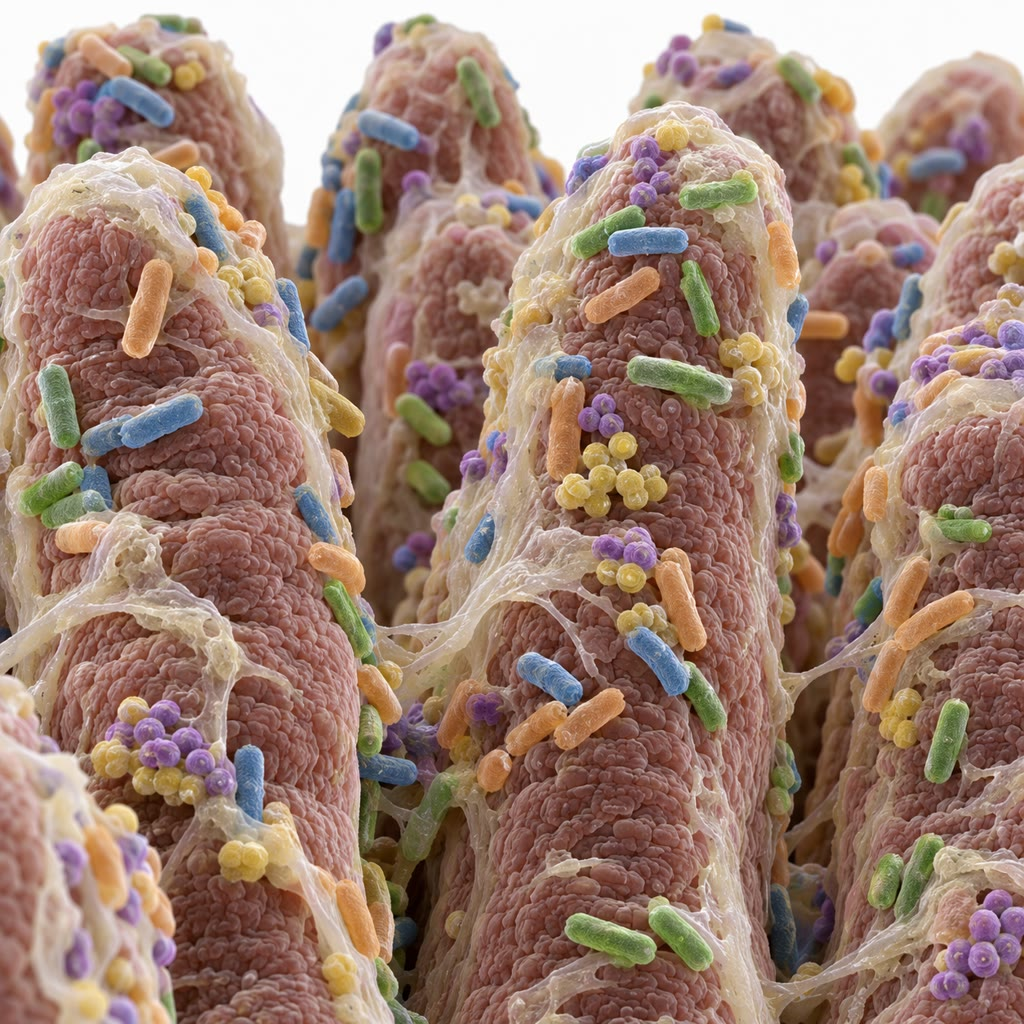
\includegraphics[width=0.40\linewidth]{images/book5/ai/b5-14-gut-microbiota.jpg}

{\small Het oppervlak van de darmbekleding in de
rasterelektronenmicroscoop, met bacteriën van verscheidene soorten in
het slijm tussen de villi.}
\end{omfigure}

\section{Planten en hun partners}

\begin{definition}[De symbiose van vlinderbloemige en rhizobium]\label{def:b3:microbiomes:nodule}
\index{rhizobia}\index{wortelknolletje}\index{Nod-factor}\index{leghemoglobine}\index{nitrogenase}
Vlinderbloemigen huisvesten stikstofbindende bacteriën
(\emph{rhizobia}) in \emph{wortelknolletjes}, organen die daarvoor
worden gebouwd na een moleculaire dialoog. De wortel scheidt
flavonoïden af; een rhizobium van de passende soort antwoordt met
\emph{Nod-factoren} --- lipochito-oligosachariden waarvan de
versieringen de partner bepalen; een receptorkinase op het wortelhaar
bindt ze en lokt schommelingen van calcium in de kern uit, het krullen
van het wortelhaar om de bacteriën heen, en een \emph{infectiedraad}
die naar binnen groeit door de cellen terwijl de schors eronder zich
tot een knolletje begint te delen. De bacteriën worden in membranen in
de knolcellen vrijgelaten en differentiëren tot \emph{bacteroïden} die
\emph{nitrogenase} tot expressie brengen, het enzym dat N$_{2}$ tot
ammoniak reduceert tegen zestien ATP per molecuul. Het nitrogenase
wordt door zuurstof vernietigd, en toch ademen de bacteroïden hard; het
knolletje lost de tegenspraak op met een diffusiebarrière en met
\emph{leghemoglobine}, een plantaardig hemoglobine dat zuurstof stevig
bindt en die bij een lage vrije concentratie naar de bacteroïden
brengt --- het is wat een doorgesneden knolletje roze maakt. De plant
betaalt zes tot tien procent van haar fotosyntheseproduct en ontvangt
het grootste deel van haar stikstof; de stikstof die de
vlinderbloemige gewassen van de wereld binden benadert die van de
kunstmestindustrie.
\end{definition}

\begin{omfigure}
\begin{tikzpicture}[every node/.style={font=\scriptsize}, >=stealth]
  % stage 1: root hair and bacteria, flavonoid / Nod factor exchange
  \begin{scope}
    \draw[thick, omMeth!60!black, fill=omMeth!15] (0,0) rectangle (1.2,3.0);
    \draw[thick, omMeth!60!black, fill=omMeth!15] (1.2,1.6) .. controls (2.4,1.7) and (2.6,2.6) .. (2.9,2.4) .. controls (2.5,2.3) and (2.3,1.4) .. (1.2,1.2) -- cycle;
    \foreach \p in {(3.1,2.7),(3.4,2.3),(3.3,1.9)} \fill[omProp] \p ellipse (0.14 and 0.07);
    \draw[->, omMeth!60!black, thick] (2.6,1.5) -- (3.2,1.4); \node[below, omMeth!60!black] at (3.0,1.35) {flavonoïden};
    \draw[<-, omProp, thick] (2.5,2.85) -- (3.0,3.0); \node[above, omProp] at (2.4,2.95) {Nod-factoren};
    \node[below, align=center] at (1.6,-0.2) {1. dialoog: wortelhaar\\en rhizobia};
  \end{scope}
  % stage 2: curled hair, infection thread
  \begin{scope}[xshift=4.6cm]
    \draw[thick, omMeth!60!black, fill=omMeth!15] (0,0) rectangle (1.2,3.0);
    \draw[thick, omMeth!60!black, fill=omMeth!15] (1.2,1.6) .. controls (2.3,1.8) and (2.8,2.6) .. (2.2,2.8) .. controls (1.9,2.9) and (1.8,2.5) .. (2.0,2.4) .. controls (2.3,2.2) and (1.9,1.3) .. (1.2,1.2) -- cycle;
    \draw[omProp, very thick] (2.05,2.55) .. controls (1.8,2.1) and (1.4,1.7) .. (0.4,1.3);
    \foreach \p in {(1.85,2.3),(1.5,1.9),(1.1,1.6),(0.7,1.4)} \fill[omProp] \p ellipse (0.1 and 0.05);
    \node[right, omProp, font=\tiny] at (2.3,1.0) {infectiedraad};
    \foreach \p in {(0.3,0.5),(0.6,0.7),(0.9,0.5)} \draw[omMeth!60!black] \p circle (0.12);
    \node[below, align=center] at (1.6,-0.2) {2. het haar krult; de draad groeit naar binnen;\\schorscellen delen};
  \end{scope}
  % stage 3: nodule
  \begin{scope}[xshift=9.0cm]
    \draw[thick, omMeth!60!black, fill=omMeth!15] (0,0) rectangle (1.2,3.0);
    \draw[thick, omThm!60!black, fill=omThm!25] (1.2,1.5) ellipse (1.3 and 1.0);
    \foreach \p in {(1.0,1.5),(1.5,1.8),(1.6,1.2),(1.1,1.9),(1.2,1.1),(2.0,1.5)} \fill[omProp] \p circle (0.1);
    \node[right, align=left] at (2.6,2.0) {knolletje: bacteroïden\\met nitrogenase};
    \node[right, align=left, omThm!60!black] at (2.6,1.1) {roze: leghemoglobine\\houdt O$_2$ laag};
    \draw[->, thick] (0.6,2.4) -- (1.0,2.0) node[pos=0, above] {suiker};
    \draw[<-, thick] (0.6,0.6) -- (1.0,1.0) node[pos=0, below] {NH$_3$};
    \node[below, align=center] at (1.6,-0.2) {3. bacteroïden binden N$_2$;\\suiker voor ammoniak};
  \end{scope}
\end{tikzpicture}

{\small Een knolletje maken. Flavonoïden van de wortel en \omterm{def:b3:microbiomes:nodule}{Nod-factoren}
van het rhizobium wijzen de partners aan; het wortelhaar krult, een
infectiedraad voert de bacteriën naar binnen, en de schors bouwt een
knolletje waarin bacteroïden, door \omterm{def:b3:microbiomes:nodule}{leghemoglobine} bij weinig zuurstof
gehouden, stikstof binden in ruil voor suiker.}
\end{omfigure}

\begin{definition}[Mycorrhiza's]\label{def:b3:microbiomes:mycorrhiza}
\index{mycorrhiza}\index{arbusculaire mycorrhiza}\index{gemeenschappelijke symbioseroute}
\emph{Mycorrhiza's} zijn verbintenissen van wortels met schimmels, te
vinden bij zo'n \qty{80}{\%} van de plantensoorten en al in de oudste
fossielen van landplanten. Bij de \emph{arbusculaire mycorrhiza's} gaat
de schimmel (een Glomeromyceet) de wortelcellen binnen en vertakt zich
tot een boomvormige arbuskel waarover fosfaat, stikstof en water naar
de plant gaan en suikers en lipiden naar de schimmel; de schimmeldraden
vergroten het opnemende oppervlak van de wortel honderdvoudig en
bereiken fosfaat waar de wortel niet bij kan. Bij de
\emph{ectomycorrhiza's} van bosbomen omhult de schimmel de wortel en
groeit zij tussen de cellen door. De plantengenen die de schimmel
binnenlaten vormen dezelfde \emph{gemeenschappelijke symbioseroute} ---
receptor, calciumpieken, transcriptiefactoren --- die de
vlinderbloemigen voor de \omterm{def:b3:microbiomes:nodule}{rhizobia} hergebruiken: het knolletje is een
late uitvinding, gebouwd op een schimmelpartnerschap dat vierhonderd
miljoen jaar ouder is.
\end{definition}

\begin{proposition}[Handel en handhaving]\label{prop:b3:microbiomes:sanctions}
\index{partnerkeuze}\index{sancties}\index{profiteur}
Een \omterm{def:b3:microbiomes:symbiosis}{mutualisme} is een ruil, en elke partner wordt geselecteerd om
minder te geven en meer te nemen; het houdt stand omdat de andere
partner kan terugslaan. Vlinderbloemigen beperken de zuurstof naar
knolletjes waarvan de \omterm{def:b3:microbiomes:nodule}{rhizobia} geen stikstof binden, wat hun
voortplanting halveert (Kiers, 2003): \emph{sancties}. Planten in
mycorrhizanetwerken geven meer koolstof aan de schimmelpartners die
meer fosfaat leveren, en de schimmels meer fosfaat aan de wortels die
meer koolstof betalen --- een markt waarin beide zijden de betere
handelaar belonen (Kiers, 2011). Inktvissen stoten bacteriën uit het
lichtorgaan die niet oplichten; het menselijke afweersysteem duldt de
commensalen die in het lumen blijven en valt die aan die de wand
oversteken. Waar een gastheer noch kan kiezen noch kan straffen --- bij
een endosymbiont die via het ei wordt geërfd --- komt het gelijklopen
van belangen in plaats daarvan uit het gedeelde lot voort: een
verticaal overgedragen symbiont plant zich alleen voort wanneer zijn
gastheer dat doet, en de selectie op de symbiont bevoordeelt de
voortplanting van de gastheer. De wijze van overdracht voorspelt dus
het karakter van de verbintenis: \omterm{def:b3:microbiomes:symbiosis}{verticale overdracht} naar \omterm{def:b3:microbiomes:symbiosis}{mutualisme}
en afhankelijkheid, horizontale overdracht naar uitbuiting die door
handhaving in toom wordt gehouden.
\end{proposition}
\admitted

\begin{omfigure}
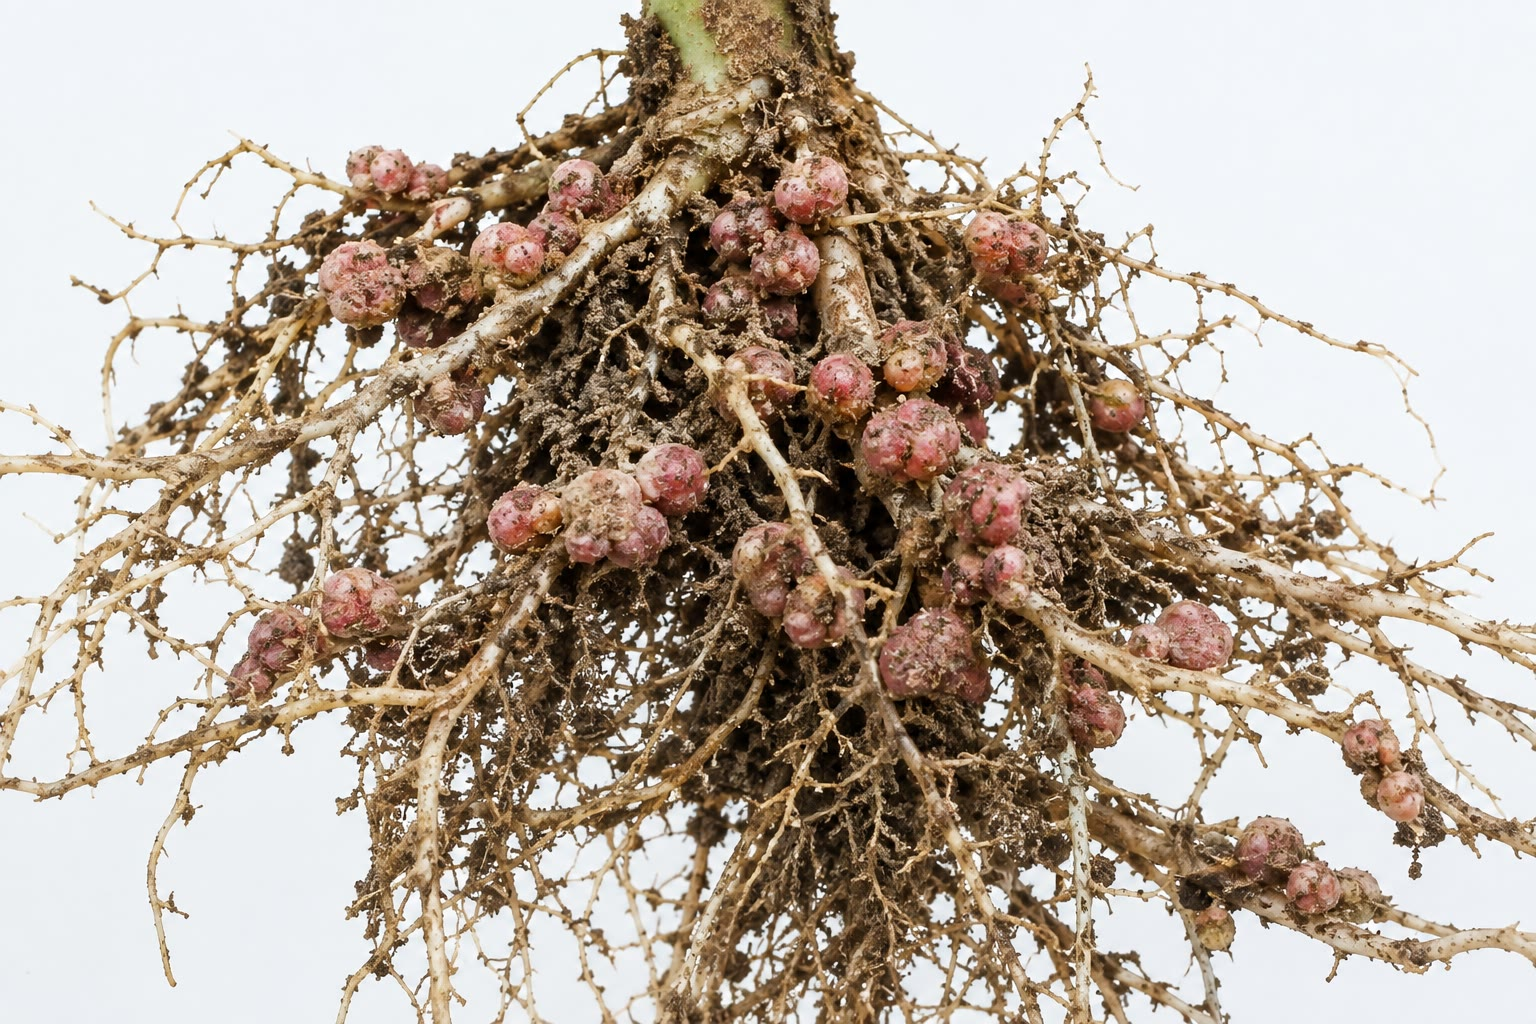
\includegraphics[width=0.46\linewidth]{images/book5/ai/b5-14-root-nodules.jpg}\hspace{0.04\linewidth}
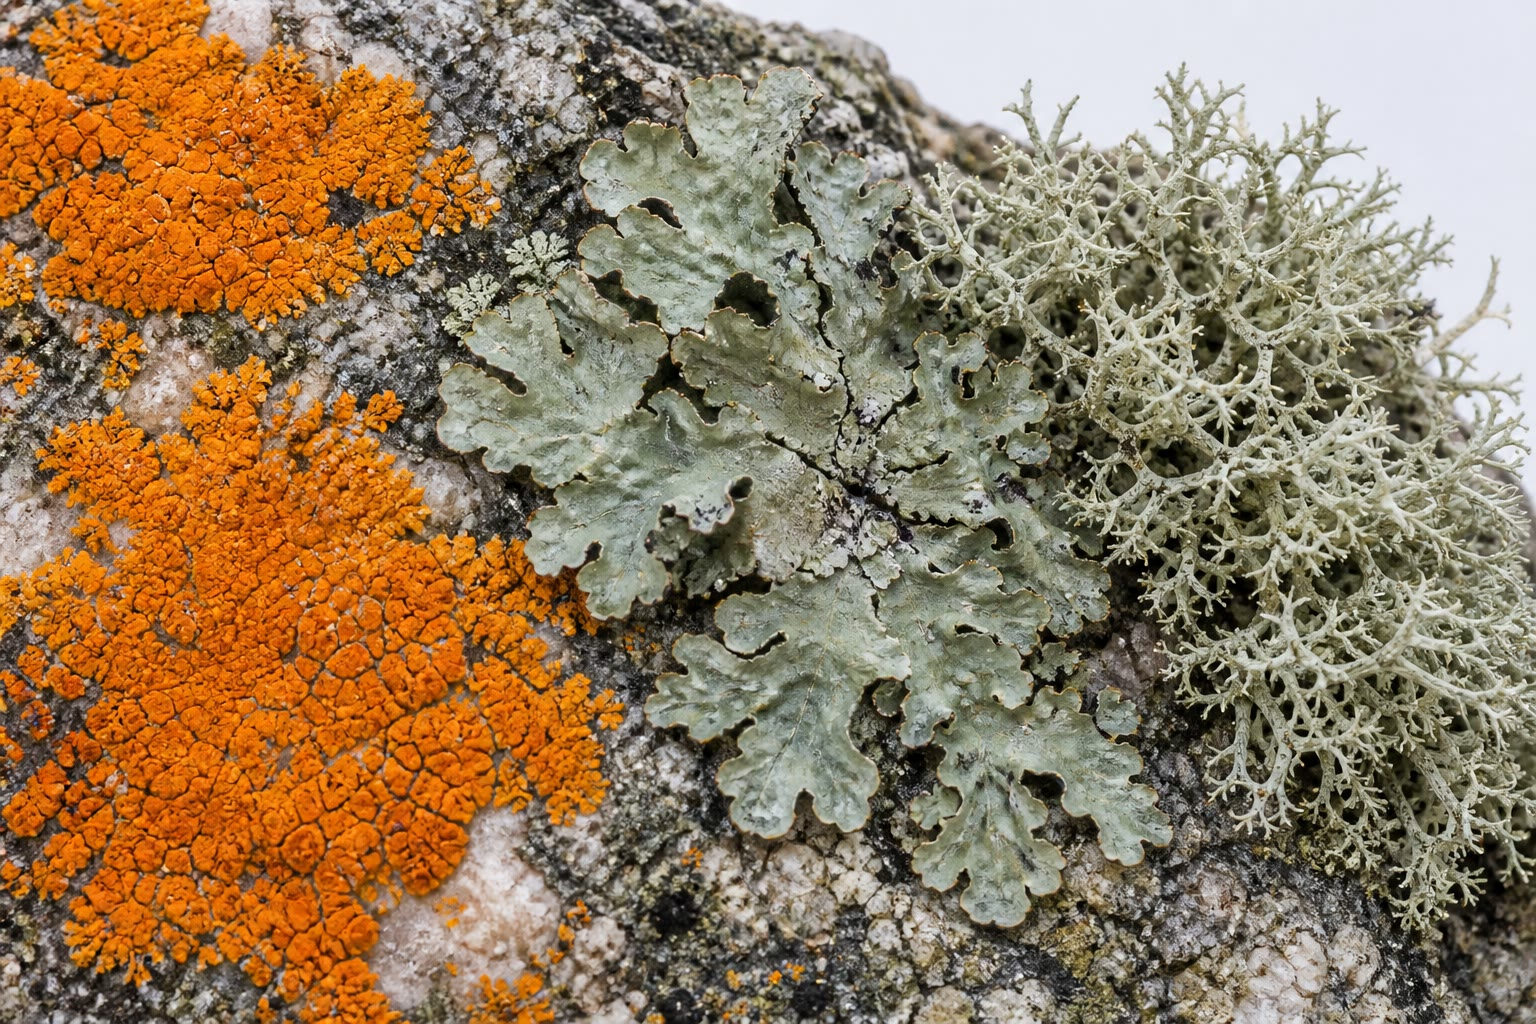
\includegraphics[width=0.46\linewidth]{images/book5/ai/b5-14-lichen.jpg}

{\small Links: de wortels met knolletjes van een vlinderbloemige, waarbij
elk roze knolletje een stikstoffabriek van bacteroïden is die met
suiker wordt gevoed. Rechts: korstmossen op steen --- elk een schimmel
die een fotosynthetische alg of cyanobacterie huisvest, samen een
oppervlak koloniserend dat geen van beide alleen zou kunnen houden.}
\end{omfigure}

\section{Verbintenissen in zee en elders}

\begin{definition}[Koraal en alg]\label{def:b3:microbiomes:coral}
\index{koraalsymbiose}\index{zoöxanthellen}\index{koraalverbleking}
Rifbouwende koralen huisvesten dinoflagellaten (de
\emph{Symbiodiniaceae}, de \emph{zoöxanthellen}) in de cellen van hun
darmbekleding, een miljoen of meer per vierkante centimeter. De algen
doen aan fotosynthese in het weefsel van het dier, met de afval-CO$_{2}$,
de ammoniak en het fosfaat van het dier, en geven tot \qty{90}{\%} van
hun gebonden koolstof terug als glycerol, suikers en aminozuren, die
het koraal en de kalkafzetting voeden die het rif opbouwt; het koraal
op zijn beurt bestuurt de stikstofvoorziening van de algen en daarmee
hun groei. De verbintenis werkt binnen een smal temperatuurvenster:
blijft het water enkele weken een tot twee graden boven het
zomermaximum, dan raakt de fotosynthese van de algen beschadigd, laten
zij reactieve zuurstof in de gastheercellen los, en stoot het koraal ze
uit --- de \emph{verbleking}, waarbij het witte skelet door het
doorschijnende dier heen schijnt. Een verbleekt koraal verhongert; het
herstelt als het water binnen weken afkoelt en sterft als dat niet
gebeurt. De frequentie van verbleking is sinds 1980 vervijfvoudigd, en
zij is het mechanisme waarmee de opwarming de riffen wegneemt.
\end{definition}

\begin{example}[Symbiosen die leefgebieden maken]\label{ex:b3:microbiomes:habitats}
Een \emph{korstmos} is een schimmel die een groenwier of een
cyanobacterie huisvest, waarbij de schimmel de structuur, het
vasthouden van water en de uit steen opgeloste mineralen levert en de
fotobiont de suiker (en, als het een cyanobacterie is, de stikstof);
korstmossen bedekken ongeveer \qty{8}{\%} van het landoppervlak,
koloniseren kaal gesteente en beginnen de omzetting ervan tot bodem. De
kokerworm \emph{Riftia} van de diepzeebronnen heeft als volwassen dier
geen mond en geen darm; hij huisvest sulfideoxiderende bacteriën in een
trofosoom en levert ze sulfide en zuurstof op een hemoglobine dat beide
bindt, en groeit in het donker op chemische energie meer dan een meter
per jaar. Termieten verteren hout met een darmgemeenschap van protisten
en bacteriën, en herkauwers verteren gras met een pens ter grootte van
een badkuip waarin bacteriën, archaea en schimmels cellulose tot
vetzuren en methaan vergisten; de koe leeft van de vetzuren en van de
lichamen van de microben zelf. In elk geval is een stofwisselend
vermogen --- fotosynthese, stikstofbinding, sulfide-oxidatie,
cellulosevertering --- dat de gastheerlijn nooit heeft ontwikkeld in
één stap door een verbintenis verworven.
\end{example}

\begin{omfigure}
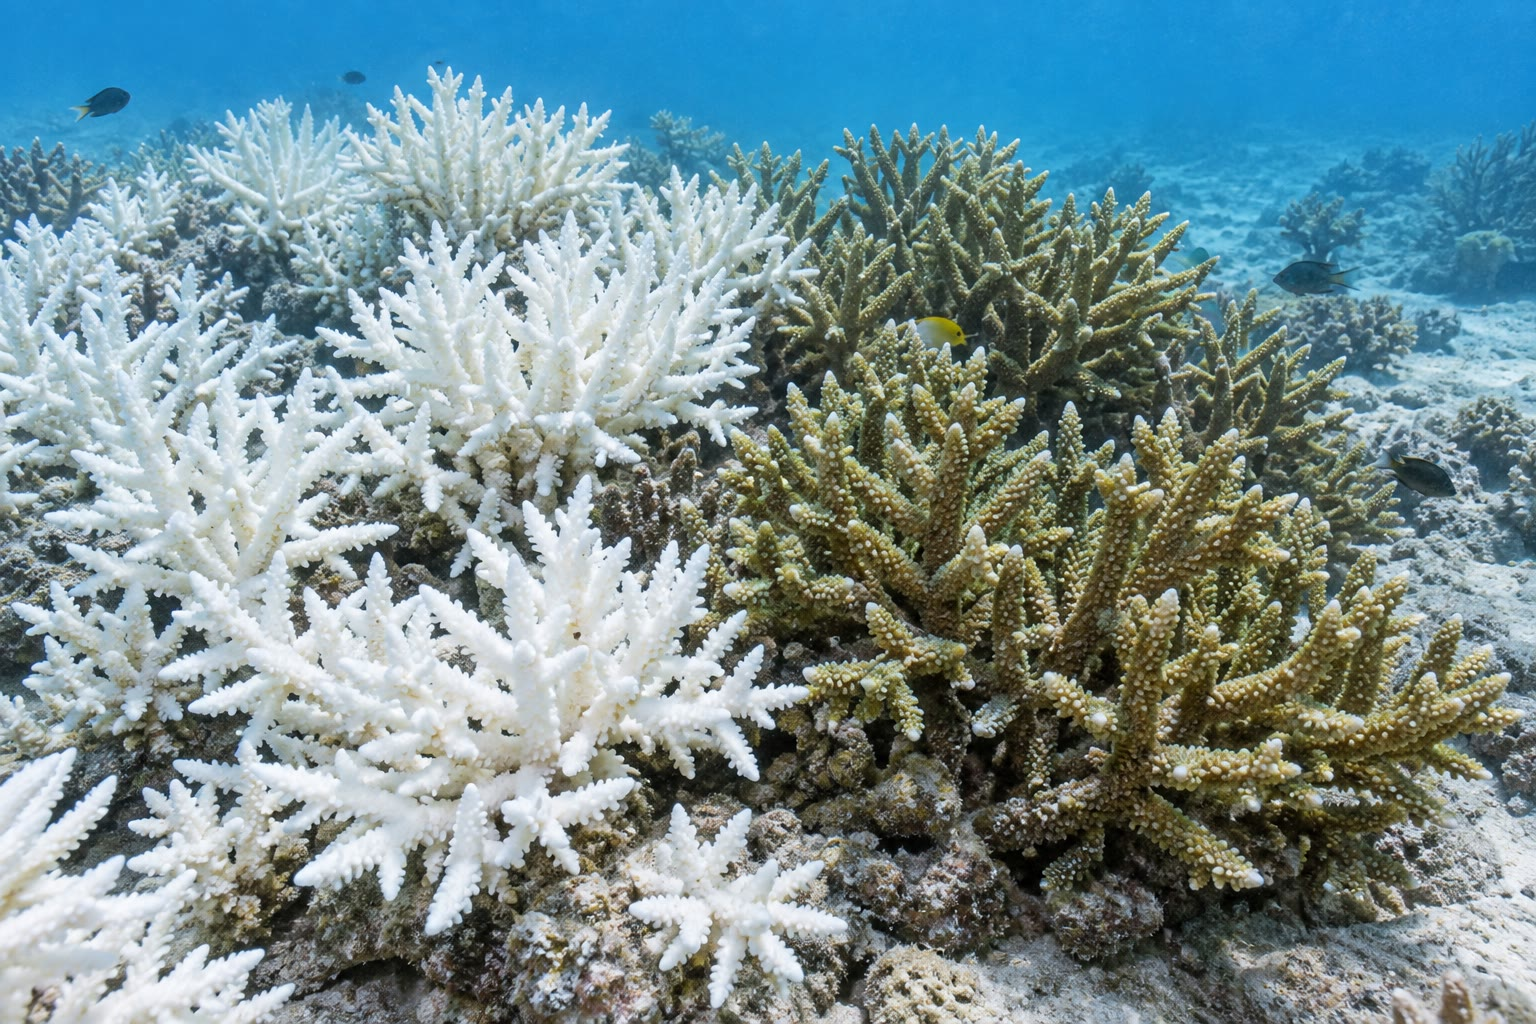
\includegraphics[width=0.56\linewidth]{images/book5/ai/b5-14-coral-bleaching.jpg}

{\small Een half verbleekt rif: de witte kolonies hebben na weken van
te warm water hun algen uitgestoten; de bruine hebben de hunne nog. Het
witte koraal leeft en verhongert, en heeft weken om opnieuw te worden
gekoloniseerd.}
\end{omfigure}

\begin{omfigure}
\begin{tikzpicture}[every node/.style={font=\scriptsize}, >=stealth]
  % coral cell with alga
  \draw[very thick, omDef, fill=omDef!8] (0,0) ellipse (3.2 and 2.0); \node[above] at (0,2.05) {koraalcel (gastrodermis)};
  \draw[thick, omMeth!70!black, fill=omMeth!30] (-0.4,-0.1) circle (1.05); \node[align=center] at (-0.4,-0.1) {alg\\(zoöxanthel)};
  % exchanges
  \draw[->, thick, omMeth!70!black] (0.5,0.4) -- (1.9,0.9) node[right, align=left] {glycerol, suikers, aminozuren:\\tot \qty{90}{\%} van de gebonden koolstof};
  \draw[<-, thick, omThm] (0.5,-0.5) -- (1.9,-1.0) node[right, align=left] {CO$_2$, NH$_3$, fosfaat\\(de afvalstoffen van het dier)};
  \draw[<-, thick, omProp] (-1.3,0.3) -- (-2.6,1.0) node[left, align=right] {licht door\\het weefsel};
  \node[below, align=center] at (1.5,-2.1) {stress: wekenlang warm water $\to$ fotosynthese beschadigd,\\reactieve zuurstof $\to$ alg uitgestoten $\to$ verbleking};
  % thermometer-like bar on the right
  \begin{scope}[xshift=7.6cm, yshift=-1.6cm]
    \draw[thick] (0,0) rectangle (0.5,3.2);
    \fill[omDef!40] (0,0) rectangle (0.5,2.0); \fill[omProp!60] (0,2.0) rectangle (0.5,2.6); \fill[omThm!60] (0,2.6) rectangle (0.5,3.2);
    \node[right] at (0.6,1.0) {normaal bereik}; \node[right] at (0.6,2.3) {$+\qty{1}{\celsius}$: stress}; \node[right, align=left] at (0.6,2.9) {$+\qty{2}{\celsius}$ wekenlang:\\verbleking};
    \node[below, align=center] at (0.25,-0.1) {zeetemperatuur\\in de zomer};
  \end{scope}
\end{tikzpicture}

{\small De ruil tussen koraal en alg: de alg bindt koolstof met de
afvalstoffen van het dier en het licht door zijn weefsel en geeft het
meeste ervan terug als voedsel; een kleine, aanhoudende stijging van de
temperatuur verbreekt de verbintenis.}
\end{omfigure}

\section{Van partner tot organel}

\begin{proposition}[Genoomkrimp en de weg naar het organel]\label{prop:b3:microbiomes:reduction}
\index{genoomkrimp}\index{endosymbiotische genoverdracht}
Een endosymbiont die via het ei wordt geërfd leeft in een populatie van
enkele cellen die nooit met buitenstaanders recombineren. De selectie
erop is zwak (\cref{ch:b3:molecular-evolution}: een kleine populatie
legt licht schadelijke mutaties door drift vast), genen waarvan de
gastheer de producten levert worden niet gemist wanneer zij kapotgaan,
en een verloren gen komt nooit terug. Het genoom krimpt daarom,
generatie na generatie --- \emph{Buchnera} tot \qty{640}{kb}, sommige
insectensymbionten tot \qty{140}{kb} en enkele honderden genen, het
mitochondrion tot \qty{16}{kb} en dertien eiwitten bij de mens --- en
de kern van de gastheer verwerft kopieën van symbiontgenen door
\emph{\omterm{prop:b3:microbiomes:reduction}{endosymbiotische genoverdracht}}, waarvan de producten met een
adressignaal weer worden ingevoerd. Zodra de gastheer de meeste
eiwitten van de symbiont maakt, zijn deling bestuurt en niet zonder
hem kan leven, is de symbiont een organel geworden. Mitochondriën en
plastiden legden deze weg twee miljard en een miljard jaar geleden af
(het boek van jaar~1); het chromatofoor van \emph{Paulinella} is een
derde reiziger, honderd miljoen jaar onderweg.
\end{proposition}

\begin{remark}[Het individu herzien]\label{rem:b3:microbiomes:individual}
Een dier of een plant is een gemeenschap met een genoom in het midden,
waarvan het grootste deel van het stofwisselende repertoire, en veel
van de ontwikkeling en de afweer, afhangt van partners die het niet in
zijn eigen DNA heeft geërfd. De praktische gevolgen zijn er al: het
\omterm{def:b3:microbiomes:symbiosis}{microbioom} als geneesmiddel (de fecestransplantatie), als doelwit van
geneesmiddelen (de nevenschade van \omterm{def:b3:bacteriology:antibiotics}{antibiotica}, voedingsvezel op
recept), als diagnostisch middel, en als weg --- via gemodificeerde
symbionten en muggen die \emph{Wolbachia} dragen --- om de biologie van
wilde populaties te veranderen. Het theoretische gevolg is dat de
natuurlijke selectie op verbintenissen ingrijpt, en dat de sterkste
verbintenissen die zijn waarin het lot van de ene partner dat van de
andere is.
\end{remark}

\section{Opgaven}

\begin{exercise}[$\star$]\label{exo:b3:microbiomes:1}
Definieer \omterm{def:b3:microbiomes:symbiosis}{mutualisme}, \omterm{def:b3:microbiomes:symbiosis}{commensalisme} en parasitisme, en geef van elk één
voorbeeld uit dit hoofdstuk. Waarom kan één paar soorten tussen de
categorieën verschuiven?
\end{exercise}

\begin{exercise}[$\star$]\label{exo:b3:microbiomes:2}
Bereken $H$, $e^{H}$, $D$ en $1/D$ voor een gemeenschap met abundanties
$0.5$, $0.3$, $0.1$, $0.05$, $0.05$.
\end{exercise}

\begin{exercise}[$\star$]\label{exo:b3:microbiomes:3}
Zet een 16S-amplicononderzoek en hagelschotmetagenomica tegenover
elkaar: wat meldt elk, en wat kan elk niet zeggen?
\end{exercise}

\begin{exercise}[$\star$]\label{exo:b3:microbiomes:4}
Noem vier diensten die het \omterm{def:b3:microbiomes:gut}{darmmicrobioom} zijn gastheer levert en één
ziekte die op de ontwrichting ervan volgt.
\end{exercise}

\begin{exercise}[$\star\star$]\label{exo:b3:microbiomes:5}
Een monster van $N = 20$ \omterm{def:b3:genomics:ngs}{reads} bevat soorten met $N_{i} = 10, 6, 3, 1$.
Bereken $E[S_{n}]$ voor $n = 5$ met de stelling, en de \omterm{thm:b3:microbiomes:rarefaction}{dekking van
Good}.
\end{exercise}

\begin{exercise}[$\star\star$]\label{exo:b3:microbiomes:6}
De dikke darm bevat \qty{400}{g} inhoud bij $10^{11}$ bacteriën per
gram; een bacterie weegt \qty{1}{pg} en haar genoom heeft \num{4000}
genen; de darm van een persoon bevat $1000$ soorten. Schat de massa van
het \omterm{def:b3:microbiomes:symbiosis}{microbioom} en het aantal verschillende genen dat het draagt, en
vergelijk met de \num{20000} van het menselijk genoom.
\end{exercise}

\begin{exercise}[$\star\star$]\label{exo:b3:microbiomes:7}
Leg de zuurstofparadox van het knolletje uit en hoe het \omterm{def:b3:microbiomes:nodule}{leghemoglobine}
en de diffusiebarrière haar oplossen. Waarom is een knolletje roze, en
wat betekent een groen knolletje?
\end{exercise}

\begin{exercise}[$\star\star$]\label{exo:b3:microbiomes:8}
Een mutante vlinderbloemige mist het onderdeel van de \omterm{def:b3:microbiomes:mycorrhiza}{gemeenschappelijke
symbioseroute} dat de calciumpieken verzorgt. Voorspel haar
knolvorming en haar mycorrhizavorming, en leg uit wat dat zegt over de
evolutie van de twee \omterm{def:b3:microbiomes:symbiosis}{symbiosen}.
\end{exercise}

\begin{exercise}[$\star\star$]\label{exo:b3:microbiomes:9}
Beschrijf het sanctie-experiment van Kiers en wat er zou worden
voorspeld als de plant fixerende en niet-fixerende knolletjes niet kon
onderscheiden.
\end{exercise}

\begin{exercise}[$\star\star\star$]\label{exo:b3:microbiomes:10}
Bewijs dat $E[S_{n}]$ uit de rarefactiestelling een stijgende functie
van $n$ is en $S$ bereikt bij $n = N$, en laat zien dat voor een soort
met $N_{i} \ll N$ en $n \ll N$ de kans om gezien te worden ongeveer
$1 - (1 - n/N)^{N_{i}}$ is.
\end{exercise}

\begin{exercise}[$\star\star\star$]\label{exo:b3:microbiomes:11}
\emph{Wolbachia} wordt alleen via eieren overgedragen. Leg uit waarom
de selectie erop vrouwelijke gastheren bevoordeelt, beschrijf de
cytoplasmatische onverenigbaarheid en laat zien waarom die een besmette
stam zich laat verspreiden zelfs als de besmetting een kleine kost met
zich meebrengt.
\end{exercise}

\begin{exercise}[$\star\star\star$]\label{exo:b3:microbiomes:12}
Leg met \cref{prop:b3:microbiomes:reduction} uit waarom de genomen van
verticaal overgedragen endosymbionten krimpen en die van hun
vrijlevende verwanten niet, welke genen het eerst en welke het laatst
verloren gaan, en wat de tendens zou omkeren.
\end{exercise}

\section{Vraagstuk: de telling van een darm}

\begin{problem}[{Weekendvraagstuk --- een darmmicrobioom geteld in
cellen, genen en calorieën, zijn diversiteit gemeten en gerarefieerd,
de stikstofbegroting van een vlinderbloemige tegen haar suiker
afgewogen, en de koolstof van een rif verantwoord, met als besluit de
calorieën die een microbioom oplevert, de dekking van een
sequencingmonster en de suiker die een bonenveld voor zijn stikstof
betaalt}]
\label{pb:b3:microbiomes:1}
Gegevens: \qty{400}{g} inhoud van de dikke darm bij $10^{11}$ bacteriën
per gram, met een celmassa van \qty{1}{pg}; $1000$ soorten, elk
\num{4000} genen, waarbij \qty{30}{\%} van de genen door elke twee
soorten wordt gedeeld. Voeding: \qty{30}{g} vezel per dag, vergist tot
kortketenige vetzuren met \qty{10}{mmol} per gram, elk \qty{0.9}{kJ}
waard; een voeding van \qty{9000}{kJ}. Een sequencingmonster: $N = 2000$
\omterm{def:b3:genomics:ngs}{reads}, $S = 180$ soorten, $f_{1} = 60$ eenlingen; abundanties van de
drie talrijkste soorten $0.30$, $0.20$, $0.10$, de rest gelijkmatig
verdeeld. Een bonengewas bindt \qty{150}{kg} N per hectare per seizoen
en betaalt \qty{8}{g} suiker per gram gebonden N; zijn fotosynthese
levert \qty{12}{t} suiker per hectare per seizoen. \omterm{def:b3:microbiomes:nodule}{Nitrogenase}: $16$ ATP
per N$_{2}$. Een koraal: $10^{6}$ algen per cm$^{2}$, die elk
\qty{20}{pg} koolstof per dag binden, waarvan \qty{90}{\%} naar de
gastheer gaat; het koraalweefsel ademt \qty{15}{\micro g} koolstof per
cm$^{2}$ per dag.

\medskip
\noindent\textbf{Deel I --- Cellen en genen.}
\begin{enumerate}
  \item Hoeveel bacteriën zitten er in de dikke darm, en wat wegen zij?
  \item Hoeveel bacteriegenomen aan DNA is dat, en hoe verhoudt het
        totaal zich tot het DNA in de $3\times 10^{13}$ menselijke
        cellen (elk \qty{6.4}{pg})?
  \item Schat het aantal verschillende bacteriegenen in de darm, met
        inachtneming van de overlap van \qty{30}{\%} (tel de niet
        gedeelde \qty{70}{\%} van elke soort plus één gedeelde
        verzameling). Vergelijk met \num{20000}.
  \item Hoeveel millimol kortketenige vetzuren levert de vezel per dag
        op, hoeveel kilojoule, en welk deel van de voeding?
  \item Een kiemvrije muis heeft \qty{30}{\%} meer voedsel nodig. Is de
        bijdrage van de vetzuren uit vraag 4 genoeg om dat te
        verklaren? Wat nog meer?
  \item Bacteriën delen zich in de dikke darm ongeveer eens per dag en
        de inhoud wordt met dezelfde snelheid geloosd. Welke
        evenwichtstoestand houdt dat in, en wat gebeurt er met de
        gemeenschap wanneer een antibioticakuur \qty{99.9}{\%} van de
        cellen doodt?
\end{enumerate}

\medskip
\noindent\textbf{Deel II --- Diversiteit.}
\begin{enumerate}[resume]
  \item Bereken de relatieve abundantie van elk van de $177$ kleine
        soorten, en daarna de \omterm{def:b3:microbiomes:diversity}{shannonindex} $H$ en $e^{H}$.
  \item Bereken de \omterm{def:b3:microbiomes:diversity}{simpsonindex} $D$ en $1/D$. Waarom is $1/D$ kleiner
        dan $e^{H}$?
  \item Wat is de \omterm{thm:b3:microbiomes:rarefaction}{dekking van Good} van het monster; hoeveel \omterm{def:b3:genomics:ngs}{reads} per
        duizend behoren tot niet-geziene soorten?
  \item Een tweede monster van \num{10000} \omterm{def:b3:genomics:ngs}{reads} uit dezelfde darm
        levert $260$ soorten op. Leg met de rarefactiestelling uit
        waarom dat geen tegenspraak is, en wat er vóór het vergelijken
        van de twee moet gebeuren.
  \item Wat is in de stelling de kans dat een soort met $N_{i} = 1$ in
        een deelsteekproef van $n = 1000$ uit $N =
        2000$ verschijnt? En bij $N_{i} = 5$?
  \item Na \omterm{def:b3:bacteriology:antibiotics}{antibiotica} toont dezelfde darm $60$ soorten, $H = 2.0$ en
        één soort met abundantie $0.5$. Bereken $e^{H}$ en $D$ en
        beschrijf de gemeenschap in woorden.
\end{enumerate}

\medskip
\noindent\textbf{Deel III --- De rekening van het knolletje.}
\begin{enumerate}[resume]
  \item Hoeveel suiker betaalt het gewas per hectare voor zijn
        \qty{150}{kg} N, en welk deel van zijn fotosynthese is dat?
  \item Hoeveel mol N$_{2}$ is \qty{150}{kg} N, en hoeveel mol ATP
        besteedt het \omterm{def:b3:microbiomes:nodule}{nitrogenase} eraan?
  \item Hoeveel kilogram glucose stelt dat ATP voor bij $30$ ATP per
        verademde glucose? Vergelijk met de betaalde suiker; waarvoor
        dient de rest?
  \item Industriële ammoniak kost ongeveer \qty{35}{MJ} per kg N.
        Vergelijk met \qty{16}{kJ} per gram suiker de energiekosten van
        de stikstof van het gewas met die van de fabriek.
  \item Een niet-fixerend rhizobium komt een knolletje binnen. Als de
        plant het straft door zijn zuurstof te halveren en zijn
        voortplanting daardoor halveert, welk deel van de \omterm{def:b3:microbiomes:nodule}{rhizobia} van
        het volgende seizoen zijn dan profiteurs, als zij bij
        \qty{10}{\%} begonnen en de fixeerders zich normaal
        voortplanten? (Eén ronde.)
  \item Zonder sancties planten profiteurs die de kosten van het
        fixeren uitsparen zich \qty{20}{\%} sterker voort. Welk deel is
        na tien seizoenen profiteur, vanaf hetzelfde begin? Wat laat de
        vergelijking zien?
\end{enumerate}

\medskip
\noindent\textbf{Deel IV --- De rekening van het rif.}
\begin{enumerate}[resume]
  \item Hoeveel koolstof binden de algen van één vierkante centimeter
        per dag, en hoeveel bereikt het koraal?
  \item Vergelijk met de ademhaling van het koraal. Wat is het
        overschot, en waarvoor wordt het gebruikt?
  \item Na de verbleking is \qty{95}{\%} van de algen weg. Herbereken de
        aangevoerde koolstof. Hoe lang kan het koraal het uithouden op
        een voorraad van \qty{300}{\micro g} koolstof per cm$^{2}$?
  \item De stress wordt vaak gemeten in graad-verhittingsweken: de som
        over het seizoen van de wekelijkse overschrijding boven het
        zomermaximum. Acht weken op $+\qty{1}{\celsius}$ of vier op
        $+\qty{2}{\celsius}$ geven beide $8$; de verbleking begint rond
        $4$. Welk van de twee verlopen is erger, en waarom kan de maat
        toch werken?
  \item Koralen kunnen verscheidene algensoorten met verschillende
        warmtegrenzen huisvesten. Stel voor hoe een rif zich zou kunnen
        aanpassen, en wat dat begrenst.
  \item Een rif met \qty{1}{km^2} levend koraaloppervlak: hoeveel
        koolstof binden zijn algen per dag en per jaar, in tonnen?
  \item Vat samen: het deel van de voeding dat het \omterm{def:b3:microbiomes:symbiosis}{microbioom} levert
        (vraag~4), de dekking van het sequencingmonster (vraag~9), en
        het deel van de fotosynthese dat een bonengewas voor zijn
        stikstof betaalt (vraag~13).
\end{enumerate}
\end{problem}
